\documentclass[tikz,border=0pt]{standalone}
\usepackage[utf8]{inputenc}
\usepackage{xcolor}

\newcommand{\cardwidth}{250pt}
\newcommand{\cardheight}{350pt}

\definecolor{cardbg}{HTML}{FFF9C0}
\definecolor{codebg}{HTML}{1A1612}
\definecolor{titlecolor}{HTML}{2D2A24}
\definecolor{bodycolor}{HTML}{4A4540}
\definecolor{categorycolor}{HTML}{888888}
\definecolor{klparen}{HTML}{888888}
\definecolor{klfunction}{HTML}{FF6B6B}
\definecolor{klstring}{HTML}{FFE66D}
\definecolor{gridcolor}{HTML}{DDDDDD}

\begin{document}
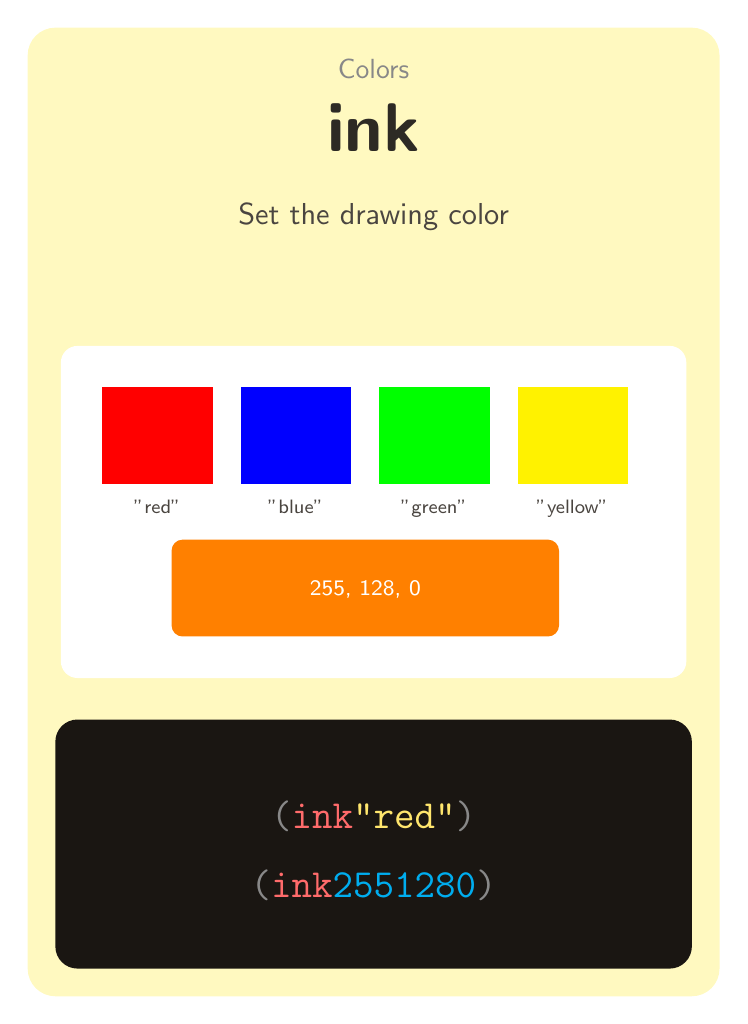
\begin{tikzpicture}
  \fill[cardbg, rounded corners=10pt] (0,0) rectangle (\cardwidth, \cardheight);
  
  \node[anchor=north, font=\sffamily\fontsize{10}{12}\selectfont\color{categorycolor}] 
    at (0.5*\cardwidth, \cardheight-8pt) {Colors};
  
  \node[anchor=north, font=\sffamily\bfseries\fontsize{28}{32}\selectfont\color{titlecolor}] 
    at (0.5*\cardwidth, \cardheight-24pt) {ink};
  
  \node[anchor=north, text width=\cardwidth-24pt, font=\sffamily\fontsize{11}{14}\selectfont\color{bodycolor}, align=center] 
    at (0.5*\cardwidth, \cardheight-60pt) {Set the drawing color};
  
  % === VISUAL DIAGRAM - Color swatches ===
  \begin{scope}[shift={(12pt, 115pt)}]
    \def\diagramwidth{226pt}
    \def\diagramheight{120pt}
    
    \fill[white, rounded corners=6pt] (0,0) rectangle (\diagramwidth, \diagramheight);
    
    % Color swatches showing ink effect
    \fill[red] (15pt, 70pt) rectangle (55pt, 105pt);
    \node[anchor=north, font=\sffamily\fontsize{7}{9}\selectfont\color{bodycolor}] at (35pt, 68pt) {"red"};
    
    \fill[blue] (65pt, 70pt) rectangle (105pt, 105pt);
    \node[anchor=north, font=\sffamily\fontsize{7}{9}\selectfont\color{bodycolor}] at (85pt, 68pt) {"blue"};
    
    \fill[green] (115pt, 70pt) rectangle (155pt, 105pt);
    \node[anchor=north, font=\sffamily\fontsize{7}{9}\selectfont\color{bodycolor}] at (135pt, 68pt) {"green"};
    
    \fill[yellow] (165pt, 70pt) rectangle (205pt, 105pt);
    \node[anchor=north, font=\sffamily\fontsize{7}{9}\selectfont\color{bodycolor}] at (185pt, 68pt) {"yellow"};
    
    % RGB example
    \definecolor{customorange}{RGB}{255,128,0}
    \fill[customorange, rounded corners=4pt] (40pt, 15pt) rectangle (180pt, 50pt);
    \node[anchor=center, font=\sffamily\fontsize{8}{10}\selectfont\color{white}] at (110pt, 32pt) {255, 128, 0};
  \end{scope}
  
  % === CODE BLOCK ===
  \fill[codebg, rounded corners=8pt] (10pt, 10pt) rectangle (\cardwidth-10pt, 100pt);
  
  \node[anchor=center] at (0.5*\cardwidth, 65pt) {
    {\fontsize{14}{18}\selectfont\ttfamily
      \textcolor{klparen}{(}%
      \textcolor{klfunction}{ink}%
      \textcolor{white}{ }%
      \textcolor{klstring}{"red"}%
      \textcolor{klparen}{)}%
    }
  };
  
  \node[anchor=center] at (0.5*\cardwidth, 40pt) {
    {\fontsize{14}{18}\selectfont\ttfamily
      \textcolor{klparen}{(}%
      \textcolor{klfunction}{ink}%
      \textcolor{white}{ }%
      \textcolor{cyan}{255}%
      \textcolor{white}{ }%
      \textcolor{cyan}{128}%
      \textcolor{white}{ }%
      \textcolor{cyan}{0}%
      \textcolor{klparen}{)}%
    }
  };
\end{tikzpicture}
\end{document}
